
\begin{figure}
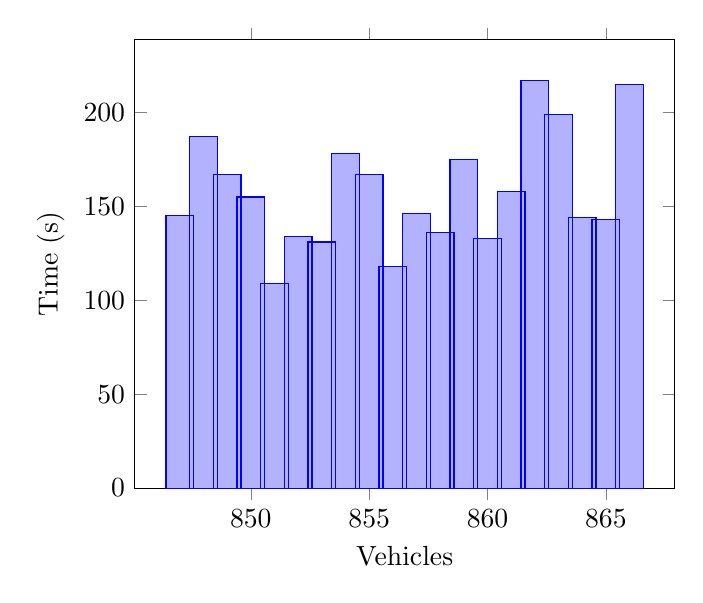
\begin{tikzpicture}
\begin{axis}[
legend style={anchor=west},
xlabel=Vehicles,
ylabel=Time (s),
ymin=0,
ybar,
]
\addplot coordinates {
(854, 178)
(856, 118)
(857, 146)
(850, 155)
(851, 109)
(852, 134)
(853, 131)
(858, 136)
(859, 175)
(848, 187)
(863, 199)
(862, 217)
(865, 143)
(864, 144)
(866, 215)
(861, 158)
(860, 133)
(855, 167)
(847, 145)
(849, 167)
};

\end{axis}
\end{tikzpicture}
\label{tik:time:100:23}
\caption{100 percent diving with GSC on route $23$}
\end{figure}
